\chapter{Tests and metrics}

After the testbed implementation, tests about its performance and metrics were
gathered in order to understand the real project effectiveness. We performed
tests relatively two main sections: one testing the architecture overall
responsivness and one checking the SFC implementation and efficiency.

\section{System responsivness}

\subsection{Docker vs Virtual Box startup measurement}

Regarding the overall system responsivness, a metric we considered worth to 
test was the VNF start up time in a docker environment versus one virtualized 
through a common virtual machine system (in this case Virtual Box was choosen). 
To make this simulation as fair as possible, we used the same node (an 
Openstack VM vith 32GB of RAM, 8 vCPU and solid state storage) and used the same 
``boot sequence'' for both the VNFs: first we launched the Astaire framework, 
ensuring it's availability to process data and then we notified the test 
machine of the successful boot. The startup time was measured from the 
beginning of the startup command (\verb!docker run! for docker and 
\verb!VBoxManage -s! for Virtual Box) till the first TCP hit received by the 
test backend (to make things as smooth as possible, \verb!netcat! was used 
to listen to incoming TCP data).

It is worth saying that Docker metrics are generally more precise than the
Virtual Box one: Docker allows to inspect the container and to gain startup and
shutdown times with a precision of millseconds, while to gather this information
for VirtualBox instances we had to use the command line utility \verb!time!,
that registered timing with a precision of hundredths of a second. Nonetheless,
this didn't influence the test too much. To avoid possible outliers we perfomed
the test $100$ times. With this $N$, the total time spent by the Virtual
Machines to boot up was of $2021,15$ seconds, while with containers the same
number of start ups resulted in a total of $1.638$. Summing up, Docker employs
only the $0,08\%$ of the overall time spent for the test, underlining how
isolating the process with a set of defined policy and avoiding a virtualized
kernel boot-up saves a considerable amount of time.

\begin{figure}[t]
    \centering
    \begin{subfigure}[b]{0.4\textwidth}
        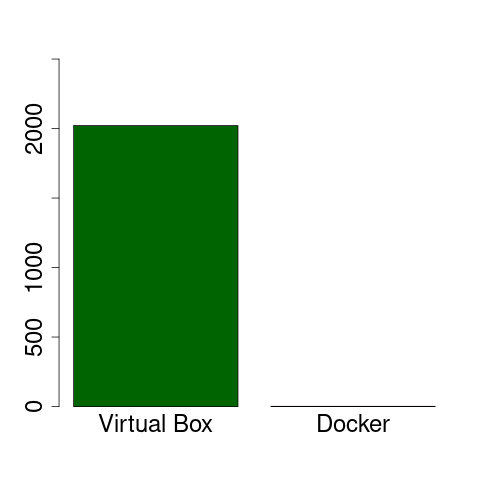
\includegraphics[scale=0.4]{docker_vs_vmBarplotGraph}
        \caption{Barplot between Virtual Box and Docker startup times.}
        \label{chap:tests:sec:dockervsvb:img:barplot}
    \end{subfigure}
    ~
    \begin{subfigure}[b]{0.4\textwidth}
        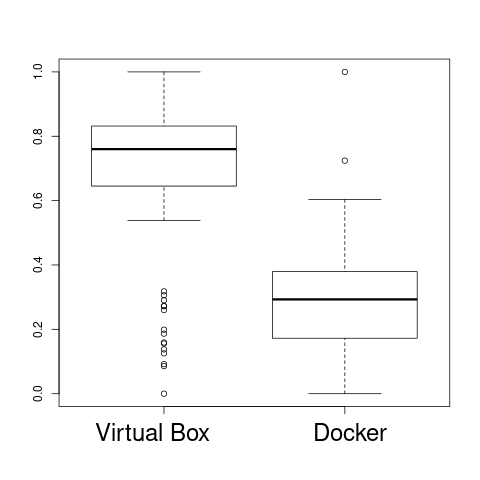
\includegraphics[scale=0.35]{docker_vs_vmBoxplotGraph}
        \caption{Boxplot between Virtual Box and Docker with values normalized 
in $0-1$ range.}
        \label{chap:tests:sec:dockervsvb:img:boxplot}
    \end{subfigure}
    \caption[Virtual Box vs Docker start up comparison]{In these graphs it is 
possible to see how the total time to start up a virtual machine through Virtual 
Box is very high compared to the time required to the overall Docker containers 
to boot. A single VirtualBox instance requires on average 20 seconds to boot up, 
while a container requires, on average, only 0.02 seconds. The main reason 
behind this difference, as already explained in other parts of this thesis, it 
is caused by the guest's kernel that has to initialized itself, before starting 
any program. On Docker, instead, the kernel is the same of the host, so the only 
operations needed are to isolate the program from the rest of the OS and add it 
to the process list.}
    \label{chap:tests:sec:dockervsvb:subimg:plots}
\end{figure}

\subsection{SFC chain deploy measurement}

The previous test make us see how much Docker is faster than a traditional
virtual machine. The test, though, was performed on a single node, interacting
directly with Docker and not through the orchestrator we used in the thesis
development, in other words Kubernetes. The following measurement will allow us
to see the time required in order to deploy an SFC of different elements in a
Kubernetes environment. The deployment consist in a Pod inside a Deployment
definition with a related Service, to simulate a real VNF. After the Pod
startup, a request is made to a backend designed to count the chain elements
that have successfully boot-up returning, eventually, the overall start up 
timing.

% TODO: missing YAML definition: [language=YAML]
%https://tex.stackexchange.com/questions/152829/how-can-i-highlight-yaml-code-in
%- a-pretty-way-with-listings
\lstinputlisting{res/code/sfc_test.yaml}

As is possible to see from the YAML definition, the test % talk about 
%imagepull policy
% Add SFC definition, graphs, talk about them
